\documentclass[12pt,a4paper]{article}
\usepackage{graphicx}
\usepackage{geometry}
\usepackage{xcolor}
\usepackage{array}
\usepackage{longtable}
\usepackage{fancyhdr}
\usepackage{amsmath}
\geometry{margin=1in}
\usepackage{array}
\setlength{\headheight}{65pt}
\begin{document}
\noindent

\begin{center}
    \Large\textbf{\color{blue}Gate -2011-IN -16 Question}
\end{center}

\thispagestyle{fancy}
\fancyhf{}
\fancyhead[L]{
\includegraphics[height=1.5cm]{IIITB-COMET-Logo.png}}
\fancyhead[R]{
\begin{tabular}{r}
\textbf{Name:DARSI VAMSI} \\
\textbf{ID: COMETFWC071} \\
\end{tabular}
}
\section*{\color{blue}QUESTION}
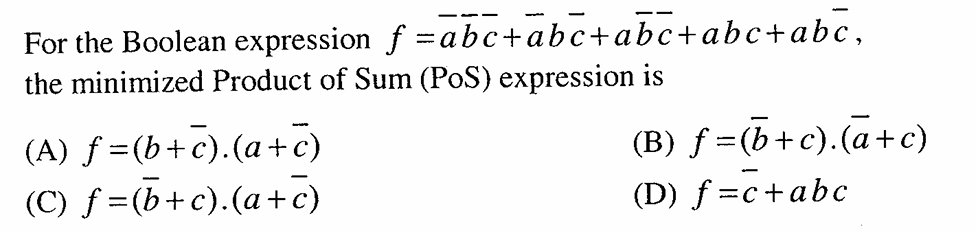
\includegraphics[width=1\textwidth,height=5 cm]{IN 2011 16-fpga.png}
\section*{\color{blue}QUESTION ANALYSIS}
\section*{Solution}

Assuming the Boolean expression is

$$
f=\bar{a}b\bar{c}+a\bar{b}\bar{c}+\bar{a}bc+abc+ab\bar{c}
$$

\subsection*{Step 1: Convert to Minterms}

$$
\bar{a}b\bar{c}=m_2
$$

$$
\bar{a}bc=m_3
$$

$$
a\bar{b}\bar{c}=m_4
$$

$$
ab\bar{c}=m_6
$$

$$
abc=m_7
$$

Therefore,

$$
f=\Sigma m(2,3,4,6,7)
$$

\subsection*{Step 2: Find the Zero Cells}

The missing minterms are

$$
m_0,\;m_1,\;m_5
$$

Hence,

$$
f=\Pi M(0,1,5)
$$

\subsection*{Step 3: K-map Grouping of Zeros}

\begin{center}
\begin{tabular}{|c|c|c|}
\hline
AB$\backslash$C & 0 & 1 \\
\hline
00 & 0 & 0 \\
\hline
01 & 1 & 1 \\
\hline
11 & 1 & 1 \\
\hline
10 & 1 & 0 \\
\hline
\end{tabular}
\end{center}

\paragraph{Group 1: $m_0$ and $m_1$}

Common variables:

$$
a=0,\qquad b=0
$$

Maxterm:

$$
(a+b)
$$

\paragraph{Group 2: $m_1$ and $m_5$}

Common variables:

$$
b=0,\qquad c=1
$$

Maxterm:

$$
(b+\bar{c})
$$

\subsection*{Step 4: Write the Minimized PoS Expression}

$$
\boxed{f=(a+b)(b+\bar{c})}
$$

\subsection*{Verification}

$$
(a+b)(b+\bar{c})
$$

is equal to 0 for

$$
000,\;001,\;101
$$

and equal to 1 for

$$
010,\;011,\;100,\;110,\;111
$$

which exactly matches the given function.

$$
\boxed{\text{Minimized PoS}=(a+b)(b+\bar{c})}
$$
\section*{Components Required}

\begin{center}
\begin{tabular}{|c|l|c|}
\hline
\textbf{S.No} & \textbf{Component} & \textbf{Quantity} \\
\hline
1 & Pygmy FPGA Board & 1 \\
\hline
2 & Seven-Segment Display & 1 \\
\hline
3 & USB Cable & 1 \\
\hline
4 & Computer/Laptop (Linux/Ubuntu/Termux) & 1 \\
\hline
5 & FPGA Toolchain (QL SymbiFlow) & 1 \\
\hline
6 & Connecting Wires (if external display is used) & As Required \\
\hline
\end{tabular}
\end{center}
\section*{Hardware Connections}

\begin{center}
\begin{tabular}{|c|c|c|}
\hline
\textbf{Pygmy FPGA Pin} & \textbf{Connected To} & \textbf{Function} \\
\hline
16 & Input A & Boolean Function Input A \\
\hline
17 & Input B & Boolean Function Input B \\
\hline
18 & Input C & Boolean Function Input C \\
\hline
20 & segment a & Seven-Segment Display Segment a \\
\hline
21 & segment b & Seven-Segment Display Segment b \\
\hline
22 & segment c & Seven-Segment Display Segment c \\
\hline
23 & segment d & Seven-Segment Display Segment d \\
\hline
25 & segment e & Seven-Segment Display Segment e \\
\hline
26 & segment f & Seven-Segment Display Segment f \\
\hline
27 & segment g & Seven-Segment Display Segment g \\
\hline
3.3V & COM Pin & Common Connection of Seven-Segment Display \\
\hline
\end{tabular}
\end{center}

\textbf{Note:} Pins 16, 17, and 18 are used as inputs corresponding to variables \(A\), \(B\), and \(C\), respectively. Pins 20--27 (excluding pin 24) are connected to the seven-segment display segments \(a\) through \(g\). The COM pin of the display is connected to the 3.3V supply.
\section*{Execution Procedure}

\begin{enumerate}

\item Create the Verilog source file \texttt{lcd_task.v} and the constraint file \texttt{lcd_task.pcf} in the working directory.

\item Compile the design using the QL SymbiFlow toolchain

\begin{verbatim}
ql_symbiflow -compile \
-d ql-eos-s3 \
-P pu64 \
-v lcd_task.v \
-t top \
-p lcd_task.pcf
\end{verbatim}

\item After successful compilation, the bitstream file is generated inside the \texttt{build} directory.

\begin{verbatim}
build/top.bit
\end{verbatim}

\item Rename the generated \texttt{.bit} file to a \texttt{.bin} file:

\begin{verbatim}
mv build/top.bit top.bin
\end{verbatim}

\item Copy the generated \texttt{.bin} file to the computer where the FPGA programming environment has been established.

\item Open a terminal and navigate to the directory containing the generated binary file:

\begin{verbatim}
cd <path_to_binary_file>
\end{verbatim}

\item Put the Pygmy FPGA board into Flash Mode and connect it to the computer using a USB cable.

\item Verify that the board is detected by the system:

\begin{verbatim}
ls -l /dev/ttyACM0
\end{verbatim}

If the device is detected, information about the serial port will be displayed.

\item Program the FPGA board using the TinyFPGA programmer utility:

\begin{verbatim}
python3 tinyfpga-programmer-gui.py \
--port /dev/ttyACM0 \
--m4app boolean_display_0.bin \
--node n4
\end{verbatim}

\item Wait until the programming process completes successfully.

\item Press the RESET button on the Pygmy FPGA board.

\item Observe the output on the hardware and verify the expected functionality.

\end{enumerate}
\section*{Results and Discussion}

The Verilog design implementing the simplified Boolean function was successfully synthesized, compiled, and programmed onto the Pygmy FPGA board. After loading the generated binary file and resetting the board, the output of the Boolean function was displayed on the seven-segment display.

For every combination of the input variables \(A\), \(B\), and \(C\), the FPGA evaluated the Boolean expression and displayed either \texttt{0} or \texttt{1} on the seven-segment display. The observed outputs matched the expected theoretical results obtained from the simplified expression.

Figure~\ref{fig:output} shows the output observed on the seven-segment display during hardware testing.

\begin{figure}[h]
\centering
% Insert captured image here
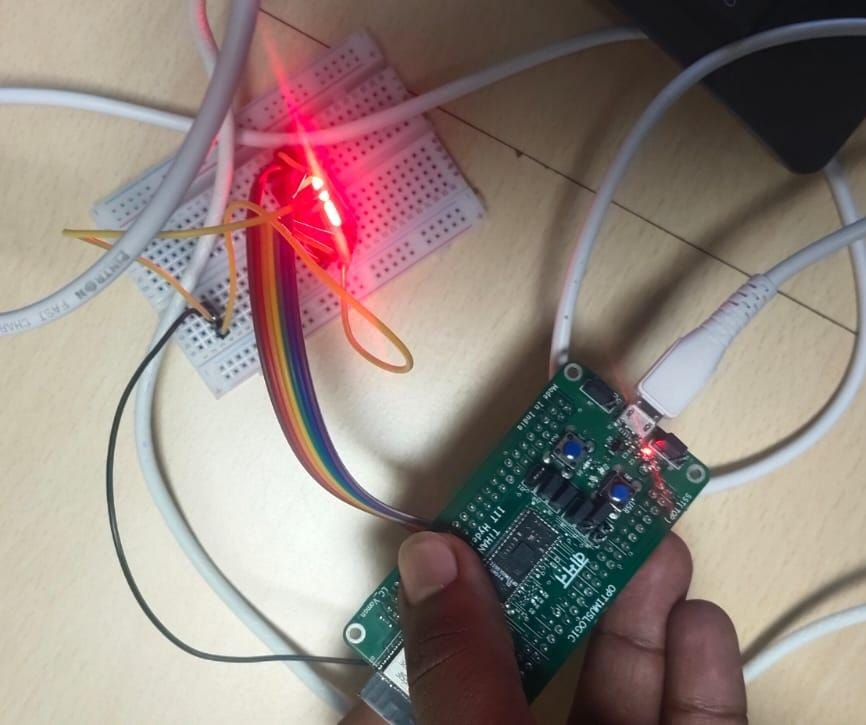
\includegraphics[width=0.5\textwidth]{7seg_lcd display output.jpeg}
\caption{Output Displayed on the Seven-Segment Display}
\label{fig:output}
\end{figure}

The truth table obtained during testing is shown below.

\begin{center}
\begin{tabular}{|c|c|c|c|}
\hline
\textbf{A} & \textbf{B} & \textbf{C} & \textbf{Displayed Output} \\
\hline
0 & 0 & 0 & 0 \\
\hline
0 & 0 & 1 & 0 \\
\hline
0 & 1 & 0 & 1 \\
\hline
0 & 1 & 1 & 1 \\
\hline
1 & 0 & 0 & 1 \\
\hline
1 & 0 & 1 & 0 \\
\hline
1 & 1 & 0 & 1 \\
\hline
1 & 1 & 1 & 1 \\
\hline
\end{tabular}
\end{center}
\end{document}